\documentclass[11pt, a4paper, twocolumn, abstract]{scrartcl}

\usepackage{geometry}
\geometry{
    textwidth=18cm, textheight=23.4cm,marginratio={1:1,5:7}      % actual formatting
    % left=1cm, right=5cm, vmargin={2.5cm,3cm}, marginparwidth=5cm   % todo-note friendly formatting (https://tex.stackexchange.com/a/156328)
}

% Table coloring stuff
\usepackage{booktabs}
\usepackage[table,xcdraw]{xcolor}
\usepackage{rotating}


% Various packages
\usepackage[utf8]{inputenc}
\usepackage{amsmath}
\usepackage[english]{babel}
\usepackage[babel]{csquotes}
\usepackage{graphicx}
\usepackage{microtype}
\usepackage{glossaries}
\newacronym{addm}{aDDM}{attentional Drift Diffusion Model}
\newacronym{glam}{GLAM}{Gaze-weighted Linear Accumulator Model}
\newacronym{aoi}{AoI}{Area of Interest}
\newacronym{bic}{BIC}{Bayesian Information Criterion}

\usepackage{abstract}

% Color links
\usepackage{xcolor}
\usepackage{hyperref}
\hypersetup{
    colorlinks,
    linkcolor={red!50!black},                           % Color of within-text links (e.g., to a Figure)
    citecolor={blue!50!black},                          % Color of citation links (within text, to Bibliography)
    urlcolor={blue!50!black}                            % Color of URLs
}


% Line numbers
%\usepackage{lineno}
%\linenumbers

% Set figure caption widths and fontsize
\usepackage{caption}
\captionsetup{
    % width=0.85\linewidth,
    font=footnotesize,
    labelfont=bf,
    labelsep=period,
    justification=justified,
    singlelinecheck=false}

\usepackage[style=apa,doi=true,url=true,eprint=false]{biblatex}
\addbibresource{references.bib}

\usepackage{authblk}

\title{Presentation order but not duration affects binary risky choice}

\author[1,2,*]{\small Felix Molter}
\author[1,2]{\small Peter N. C. Mohr}
\affil[1]{\footnotesize School of Business \& Economics, Freie Universität Berlin, Berlin, Germany}
\affil[2]{\footnotesize Center for Cognitive Neuroscience, Freie Universität Berlin, Berlin, Germany}
\affil[*]{\footnotesize E-mail: \href{mailto:felixmolter@gmail.com}{felixmolter@gmail.com}}

\date{\today}

\begin{document}

%TC:ignore
\twocolumn[
\maketitle

% Abstract
% ========
\begin{onecolabstract}
Risky choice behaviour often deviates from the predictions of normative models. The information search process has been suggested as a source of some reported "biases".
Specifically, gaze-dependent evidence accumulation models, where unfixated alternatives' signals are discounted, propose a mechanistic account of observed associations between eye movements, choices and response times, with longer fixated alternatives being chosen more frequently.
It remains debated, however, whether gaze causally influences the choice process, or rather reflects emerging preferences. Furthermore, other aspects the information search process, like the order in which information is inspected, can be confounded with gaze duration, complicating the identification of their causal influences.
In our preregistered study 179 participants made repeated incentivized choices between two sequentially presented risky gambles, allowing the experimental control of presentation duration, order, and format (i.e., alternative-wise or attribute-wise). Across presentation formats, we find evidence against an influence of presentation duration on choice. The order in which participants were shown stimulus information, however, causally affected choices, with alternatives shown last being chosen more frequently.
Notably, while gaze-dependent accumulation models generally capture effects of gaze duration, causal effects of stimulus order are only predicted by some models, identifying potential for future theory development. 
\bigskip
\end{onecolabstract} 
%TC:endignore
% Sci Reports: 200 words
]

% Main text
% =========

% Introduction
% ------------
\section*{Introduction} % around 1272 words
% Limits
% Sci Reports: Main text (excluding methods, abstract, references, figures) = Intro Results Discussion no more than 4500

A large body of experimental research demonstrates that human risky choices systematically differ from those predicted by optimal, utility-maximising and context-invariant theories of choice like Expected Utility Theory \parencite[e.g.,][]{allais1953ExtensionTheoriesEquilibre,kahneman2012ChoicesValuesFrames,mohr2017AttractionEffectRisky,molter2021GazedependentEvidenceAccumulation,hertwig2004DecisionsExperienceEffect}.
Many descriptive theories of risky choice ascribe these departures to perceptual or attentional processes \parencite[e.g.,][]{tversky1992AdvancesProspectTheory,busemeyer1993DecisionFieldTheory,yechiam2013LossaversionLossattentionImpact}, with the idea that the decision maker's capacity to process information is limited, and attention serves to select and amplify information about the choice setting (e.g., different alternatives' attributes, outcomes, or their probabilities). This selection and weighting of information is then assumed to induce biases in the decision process and ultimately affect the choice itself. 

While the specific construct of attention differs between theories and its usefulness as a general explanatory device has been questioned \parencite{hommel2019NoOneKnows}, eye movements are often taken as an indicator of which information a decision maker processes during the decision. The most ubiquitous finding in eye tracking studies of decision-making (including risky choices) is that alternatives that are looked at longer are more likely to be chosen \parencite{stewart2016EyeMovementsRisky,stewart2016EyeMovementsStrategic,cavanagh2014EyeTrackingPupillometry,isham2013LookingTimePredicts,krajbich2010VisualFixationsComputation,krajbich2011MultialternativeDriftdiffusionModel,gluth2018ValuebasedAttentionalCapture,gluth2020ValuebasedAttentionNot,sepulveda2020VisualAttentionModulates,lopez-persem2016HowPriorPreferences,thomas2019GazeBiasDifferences,thomas2021UncoveringComputationalMechanisms,molter2021GazedependentEvidenceAccumulation,smith2018AttentionChoiceDomains,ashby2016FindingRightFit,glockner2011EyetrackingStudyInformation,fiedler2012DynamicsDecisionMaking}. Gaze-dependent accumulation models \parencite{krajbich2010VisualFixationsComputation,krajbich2011MultialternativeDriftdiffusionModel,krajbich2012AttentionalDriftdiffusionModel,glickman2019FormationPreferenceRisky} provide a formal account of this \emph{gaze bias} effect and many other details of the empirical association between gaze and choice. They assume that decisions are made by repeated sampling and accumulation of evidence in favour of each alternative until evidence for one alternative reaches a decision threshold. Crucially, accumulation is assumed to depend on gaze allocation, such that information momentarily outside of the decision maker's gaze is discounted. 
Notably, gaze-dependent accumulation can explain departures from rational choice \parencite{gluth2018ValuebasedAttentionalCapture,molter2021GazedependentEvidenceAccumulation}, providing theories positing broad attentional effects on choice with concrete process-based evidence.

There remains, however, the question of causality: It is still debated to what extent eye movements causally influence the choice process (and visual attention has a causal role in choice and choice biases), or if they merely reflect an emerging choice \parencite{mormann2021DoesAttentionIncrease,westbrook2020DopaminePromotesCognitive}. Note that the accuracy with which gaze-dependent accumulation models predict choices and process measures does not address the issue of causality. Even though these models are frequently interpreted to assume a directed effect of gaze on choice, they only formalize the association between gaze and the choice process, without any directional assumption of causality. For example, it would still be possible for a third variable to influence both choices and gaze. Identifying the direction of causality ultimately requires experimental manipulation.

This issue is of great interest, as a causal effect of gaze on choice would imply that decisions could be influenced by irrelevant, external factors that affect the decision makers' gaze.

Prior work has investigated different aspects in which changes to the information search process affect choice behaviour, experimentally controlling the perceptual saliency of attributes or alternatives \parencite{weber1997ReasonsRankDependentUtility,milosavljevic2012RelativeVisualSaliency}, the duration for which alternatives or attributes were seen \parencite{armel2008BiasingSimpleChoices,shimojo2003GazeBiasBoth,tavares2017AttentionalDriftDiffusion,parnamets2015BiasingMoralDecisions,liu2020ExploitingDynamicsEye,sui2020TimingGazecontingentDecision,lim2011DecisionValueComputations}, the temporal order in which alternatives are inspected \parencite{liu2020PowerLastFixation}, or the direction in which decision makers can gather information about alternatives and their attributes \parencite{reeck2017SearchPredictsChanges, mittone2020InducingAlternativebasedCharacteristicbased}:

Gaze-dependent accumulation models of risky choice predict that a longer gaze towards an alternative is associated with a higher probability of choosing it \parencite[unless its value is aversive; see][]{smith2019GazeAmplifiesValue}. If the effect of gaze on choice was causal, this would imply that experimentally inducing longer gaze towards one choice alternative should increase its likelihood of being chosen.
A recent study found support for this effect in risky choices using a gaze-contingent decision prompt paradigm, where participants are free to inspect choice alternatives, but are prompted to make their decision when their viewing patterns favour a target attribute or alternative \parencite{sui2020TimingGazecontingentDecision}. Convergent findings have been reported in other decision-making domains \parencite{parnamets2015BiasingMoralDecisions,tavares2017AttentionalDriftDiffusion,liu2020ExploitingDynamicsEye,armel2008BiasingSimpleChoices,shimojo2003GazeBiasBoth}.

Similarly, as predicted by some gaze-dependent accumulation models \parencite{glickman2019FormationPreferenceRisky} longer relative gaze towards individual attributes (e.g., outcomes or probabilities) is associated with changes in choice behaviour \parencite{kim2012PreferenceReversalsDecision,glickman2019FormationPreferenceRisky}, and there is initial evidence that the effect is causal, too \parencite{liu2020ExploitingDynamicsEye}. These results are in line with other studies that, while not controlling gaze duration, found that manipulation of attribute salience affected choices accordingly \parencite{weber1997ReasonsRankDependentUtility}.

Apart from the duration for which alternatives and attributes were evaluated, the temporal order in which information is processed has also been associated with choice. In particular, the last fixation before a choice is often directed towards the chosen alternative. Again, however, the causal direction of this association is debated.
The gaze cascade theory \parencite{shimojo2003GazeBiasBoth} argues that this finding results from reciprocal positive feedback loops between valuation and information search processes, such that preferred alternatives are attended more, which in turn increases preference for them.
Order effects are also captured by multiple computational theories of decision making, albeit in different ways: In the \gls{addm} \parencite{krajbich2010VisualFixationsComputation,krajbich2011MultialternativeDriftdiffusionModel} this phenomenon is explained by the fact that fixated alternatives are more likely to cross the threshold, as evidence for other alternatives is discounted. Other than this, however, the model does not assume a special role of the last fixation, or the serial position of any piece of inspected information. \textcite{mullett2016ImplicationsVisualAttention} showed that an increasing association between gaze and choice before a decision is made, naturally emerges in some gaze-dependent accumulation models and does not imply preference-driven information search.
Nevertheless, \textcite{liu2020PowerLastFixation} found that manipulating which of two snack food items was shown last before a decision is prompted causally biased choices in favor of this item. 
Other models \parencite{glickman2019FormationPreferenceRisky,ashby2016FindingRightFit} assume a leaky integration process that weighs information acquired later in the decision more heavily, and thereby predicts recency effects such that later presented information should affect choices more strongly. Empirical evidence for recency effects in risky choices comes from decisions from experience \parencite{hertwig2004DecisionsExperienceEffect}, where participants learn about alternatives' properties by repeated sampling and related work on value integration in a rapidly presented stream of option outcomes \parencite{tsetsos2012SalienceDrivenValue}.

Recent work in multiattribute decisions found that the time point at which information about one attribute dimension is considered in a decision affects choice \parencite{maier2020DissociableMechanismsGovern,sullivan2021HealthfulChoicesDependa,amasino2019AmountTimeExert}. In contrast to a simple recency effect, however, these models predict that attributes considered earlier than others exert more influence on the choice process, as this also implies a longer total duration of consideration. These results further highlight the important issue that duration and order effects can be closely related (i.e., last seen alternatives are often also seen longer; and both factors are associated with choice) and need to be distinguished carefully.

% Figure 0: Visualization of hypotheses
\begin{figure}[tb]
    \centering
    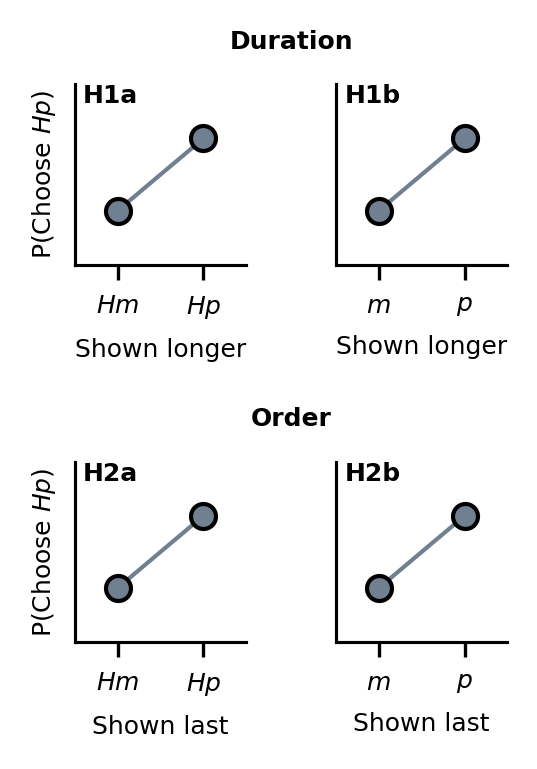
\includegraphics[width=0.9\columnwidth]{figures/hypotheses.png}
    \caption{Hypothesized qualitative effects. \textbf{H1a}: Higher probability of choosing the alternative with the higher probability ($Hp$) when it is shown longer. \textbf{H1b}: Higher probability of choosing $Hp$ when probabilities are shown longer. \textbf{H2a}: Higher probability of choosing $Hp$ when it is shown last. \textbf{H2b}: Higher probability of choosing $Hp$ when probabilities are shown last. }
    \label{fig:hypotheses}
\end{figure}

% Summary of study
Here, we add to this body of research and jointly investigate these multiple potentially causal effects of the information search (presentation duration and order) on choice. We performed a preregistered study using a task that involved incentivized choices between two risky gambles, and was designed to investigate the independent contributions of presentation duration and order to and possible interactions in the choice process. Notably, we tested the duration and order effects on two levels, namely, the level of alternatives and the level of attribute dimensions.

% Hypotheses
Specifically, we hypothesized that presentation \emph{duration} affects choices in two ways: First, in line with gaze-dependent accumulation models, longer presented alternatives should be chosen more frequently (Figure \ref{fig:hypotheses} H1a). In addition, we hypothesized that alternatives with higher values on longer presented attributes are chosen more frequently (Figure \ref{fig:hypotheses} H1b).
Analogously, we hypothesized that presentation \emph{order} affects choices, such that alternatives presented last (Figure \ref{fig:hypotheses} H2a), and alternatives with higher values on the attribute presented last (Figure \ref{fig:hypotheses} H2b) are chosen more frequently. Our preregistration contained an additional hypothesis and corresponding analysis concerning presentation-dependent changes in value-integration. Details are reported in the \nameref{sec:supplement}.

% Brief summary of results
In contrast to our predictions and prior literature, our data supports null effects of presentation duration in both attribute- and alternative-wise presentation formats. Instead, we find a causal effect of presentation order on choice, such that alternatives shown last were more likely to be chosen. We discuss the implications of these results.

% Figure 1: Choice task and stimuli
\begin{figure*}[t!]
    \centering
    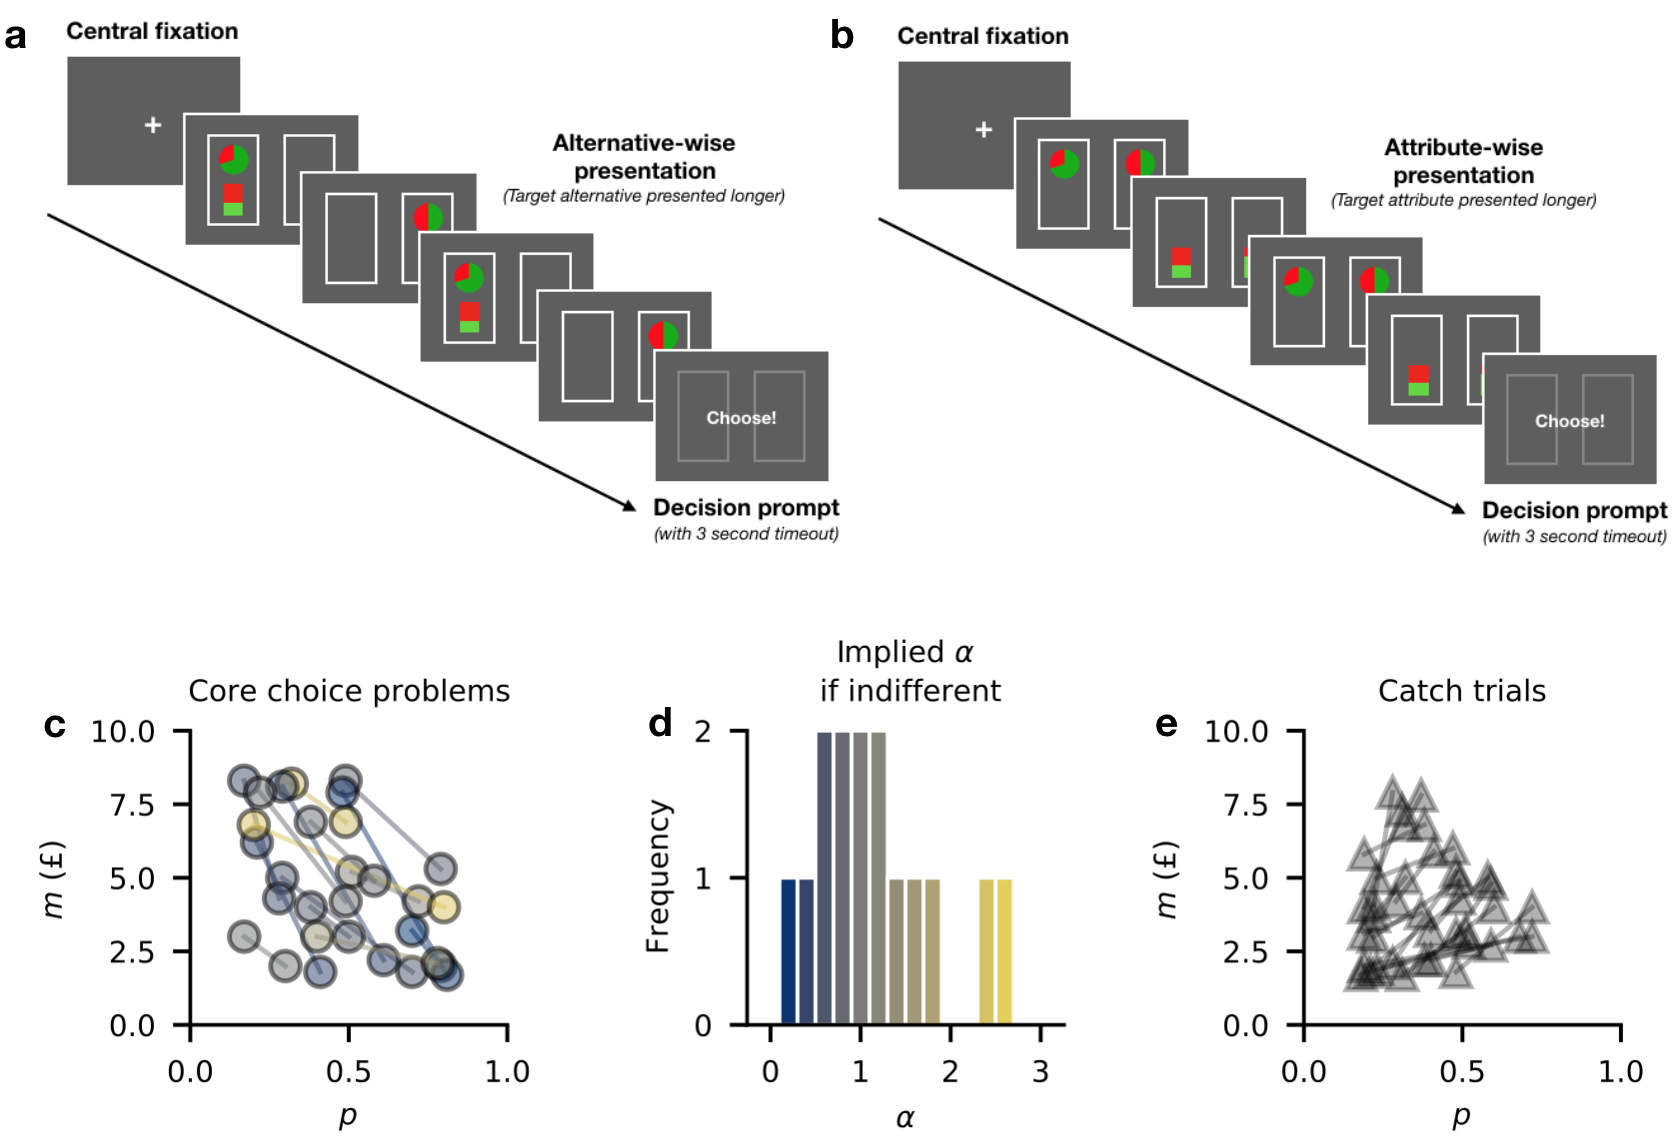
\includegraphics[width=0.9\textwidth]{figures/task_and_stimuli.png}
    \caption{Sequential presentation risky choice task and choice problems. In each trial, participants decided between two all-or-nothing gambles representing the probability $p$ to win an amount $m$. Information was presented sequentially across four stages so that total presentation duration and presentation order of alternatives (in alternative-wise presentation; \textbf{a)} or attributes (in attribute-wise presentation; \textbf{b)}) was controlled. After the presentation, participants had 3 seconds to indicate their choice. In each trial, the target alternative or attribute was shown longer than the other. \textbf{c)} 15 core choice problems used to construct choice trials. Each circle represents one choice alternative, described by its probability $p$ and outcome $m$. Each connected pair of circles indicates one pair of choices used to construct the 120 experimental trials. Color indicates the $\alpha$ value for which the expected utilities of a pair are equal (see panel \textbf{d}). \textbf{d)} Distribution of indifference implied $\alpha$ values of the 15 core choice problems from \textbf{c}). \textbf{e)} Catch trials. Each connected pair of triangles represents one of 20 catch trials, where one alternative is dominated by the other on both attributes.}
    \label{fig:taskstimuli}
\end{figure*}

% Results
% -------
\section*{Results}

\subsection*{Behavioural task}

In our experiment, 179 participants performed a binary sequential presentation risky choice task (Figure \ref{fig:taskstimuli}), where they made repeated choices between two all-or-nothing risky gambles: One alternative offering a high chance to win a smaller amount ($Hp$) and a second alternative offering a higher amount with a lower probability ($Hm$). Each trial consisted of a presentation phase, where participants learned about the two alternatives' winning probabilities $p$ and outcomes $m$, and a choice phase. Information was presented across four stages either alternative-wise (Figure \ref{fig:taskstimuli}a) or attribute-wise (Figure \ref{fig:taskstimuli}b). We experimentally controlled presentation duration and order in the task: In each trial one alternative (in alternative-wise presentation) or attribute (in attribute-wise presentation) was shown longer than its competitor (3 vs. 2 seconds across the four stages). In addition, alternatives or attributes could be shown first and third, or second and last in the sequence. In total, participants performed 120 experimental trials based on 15 core choice problems (Figure \ref{fig:taskstimuli}c, d), and 20 additional catch trials with a dominant alternative (Figure \ref{fig:taskstimuli}e). See \nameref{sec:methods} for additional details on the behavioural task and stimuli.

\subsection*{Choice behaviour summary}

% Report:
% Mean ± s.d. and range of counts of choices of dominated / dominating alternatives in catch trials (after removing participants for making too many of those choices) to show that they understood the task
Participants successfully avoided choosing dominated alternatives in catch trials (average $\pm$ s.d. count of dominated choices = 0.35 $\pm$ 0.83) with a majority of 140 participants (79\%) never choosing a dominated alternative.

% Mean ± s.d. and range of P(choose Hp) in experimental trials to illustrate that only few participant simply always chose safe or money
In experimental trials, only three participants (1.7\%) exclusively chose the $Hp$ (two participants) or $Hm$ (one participant) alternatives. All other participants alternated between alternatives to varying degrees, indicating that the selected choice problems covered individual indifference points between high and low probability gambles for a majority of participants (overall mean $\pm$ s.d. P(choose $Hp$) = 0.62 $\pm$ 0.20; Table \ref{tab:choiceprobs}).


% Table 1: Choice frequencies for Hp across conditions
% (3 decimal places)
% \begin{table}[bt!]
% \begin{tabular}{@{}llllll@{}}
% \toprule
% Presentation by & \multicolumn{2}{l}{Alternatives} & \multicolumn{2}{l}{Attributes} &    All \\ \midrule
% Duration favours &     $Hm$ & $Hp$ &   $Hm$ & \multicolumn{2}{l}{$Hp$}        \\
% Last stage favours &              &          &            &          &        \\
% $Hm$               &        0.602 &    0.602 &      0.612 &    0.620 &  0.609 \\
% $Hp$               &        0.635 &    0.630 &      0.642 &    0.626 &  0.633 \\ \midrule
% All                &        0.618 &    0.616 &      0.627 &    0.623 &  0.621 \\
% \bottomrule
% \end{tabular}
% \caption{Mean choice probabilities for the high probability alternative $Hp$ across conditions.}
% \label{tab:choiceprobs}
% \end{table}

% (2 decimal places)
\begin{table}[bt!]
\begin{centering}
\begin{tabular}{@{}llllll@{}}
\toprule
Presentation by & \multicolumn{2}{l}{Alternatives} & \multicolumn{2}{l}{Attributes} &    All \\ \midrule
Duration favours &     $Hm$ & $Hp$ &   $Hm$ & \multicolumn{2}{l}{$Hp$}        \\
Last stage favours &              &          &            &          &        \\
$Hm$               &        0.60 &    0.60 &      0.61 &    0.62 &  0.61 \\
$Hp$               &        0.64 &    0.63 &      0.64 &    0.63 &  0.63 \\ \midrule
All                &        0.62 &    0.62 &      0.63 &    0.62 &  0.62 \\
\bottomrule
\end{tabular}
\caption{Mean choice probabilities for the high probability alternative $Hp$ across conditions.}
\label{tab:choiceprobs}
\end{centering}
\end{table}

\subsection*{Regression analysis: Effect of presentation order, but not duration}

% Table 2: Regression analysis results
\begin{table*}[tb!]
	\centering
	{
		\begin{tabular}{lrrrrrrr}
			\toprule
			\multicolumn{1}{c}{} & \multicolumn{1}{c}{} & \multicolumn{1}{c}{} & \multicolumn{2}{c}{95\% HDI} & \multicolumn{1}{c}{} & \multicolumn{1}{c}{} & \multicolumn{1}{c}{} \\
			\cline{4-5}
			Term & Mean & SD & Lower & Upper & $\hat{R}$ & ESS (bulk) & ESS (tail)  \\
			\cmidrule[0.4pt]{1-8}
			\textbf{Intercept} & 0.35 & 0.11 & 0.12 & 0.56 & 1.00 & 351 & 586  \\
			\textbf{EV diff.} ($Hp - Hm$; z-scored) & 1.96 & 0.10 & 1.77 & 2.15 & 1.00 & 763 & 1962  \\
			Duration ($Hp$ or $p$ longer) & $-0.02$ & 0.04 & $-0.10$ & 0.05 & 1.00 & 8644 & 6667  \\
			\textbf{Order} ($Hp$ or $p$ last) & 0.17 & 0.04 & 0.09 & 0.25 & 1.00 & 7602 & 6943  \\
			Format (by alt.) & $-0.06$ & 0.04 & $-0.13$ & 0.01 & 1.00 & 10598 & 6192  \\
			Duration $\times$ Format & 0.01 & 0.08 & $-0.13$ & 0.16 & 1.00 & 9983 & 6276  \\
			Order $\times$ Format & 0.09 & 0.08 & $-0.06$ & 0.23 & 1.00 & 10963 & 6350  \\
			\bottomrule
		\end{tabular}
	}
	\caption{\textbf{Fixed effects estimates from Bayesian mixed-effects logistic regression.} Dependent variable: $Hp$ choice. Categorical predictors (Duration, Order, Format) were effect-coded, and positive estimates are associated with the level indicated in parentheses. See \nameref{sec:methods} for details on predictor variables. ESS: Effective sample size. Results obtained from two MCMC chains with 5000 posterior samples and 1000 tuning samples. Terms credibly different from zero are shown in boldface.}
	\label{tab:regression}
\end{table*}

We first analysed choice behaviour using a Bayesian mixed-effects logistic regression model, predicting choice from differences in expected value and effect-coded predictors indicating presentation format, the alternative favoured by presentation duration, the alternative favoured by the last presentation stage, and interaction terms of the duration and order effects with the presentation format (see \nameref{sec:methods}; Table~\ref{tab:regression}).

Choices were strongly driven by the difference in expected value ($\beta = 1.96$ $[1.77, 2.15]$) such that alternatives with higher expected values were preferred. In addition, the main effect of presentation order was credibly positive ($\beta = 0.17$ $[0.09, 0.25]$) indicating a preference towards alternatives favoured by information shown last. No other main or interaction effect was credibly different from zero (presentation duration $\beta = -0.02$ $[-0.10, 0.05]$; presentation format $\beta = -0.06 [-0.13, 0.01]$; duration-by-format interaction $\beta = 0.01$ $[-0.13, 0.16]$; order-by-format interaction $\beta = 0.09$ $[-0.06, 0.23]$). 

Next, we addressed our hypotheses regarding effects of presentation duration and order on choice separately, using preregistered directed Bayes factor $t$-tests and BEST analyses.

\subsection*{No effects of presentation duration across presentation formats}

\begin{figure*}[t]
    \centering
    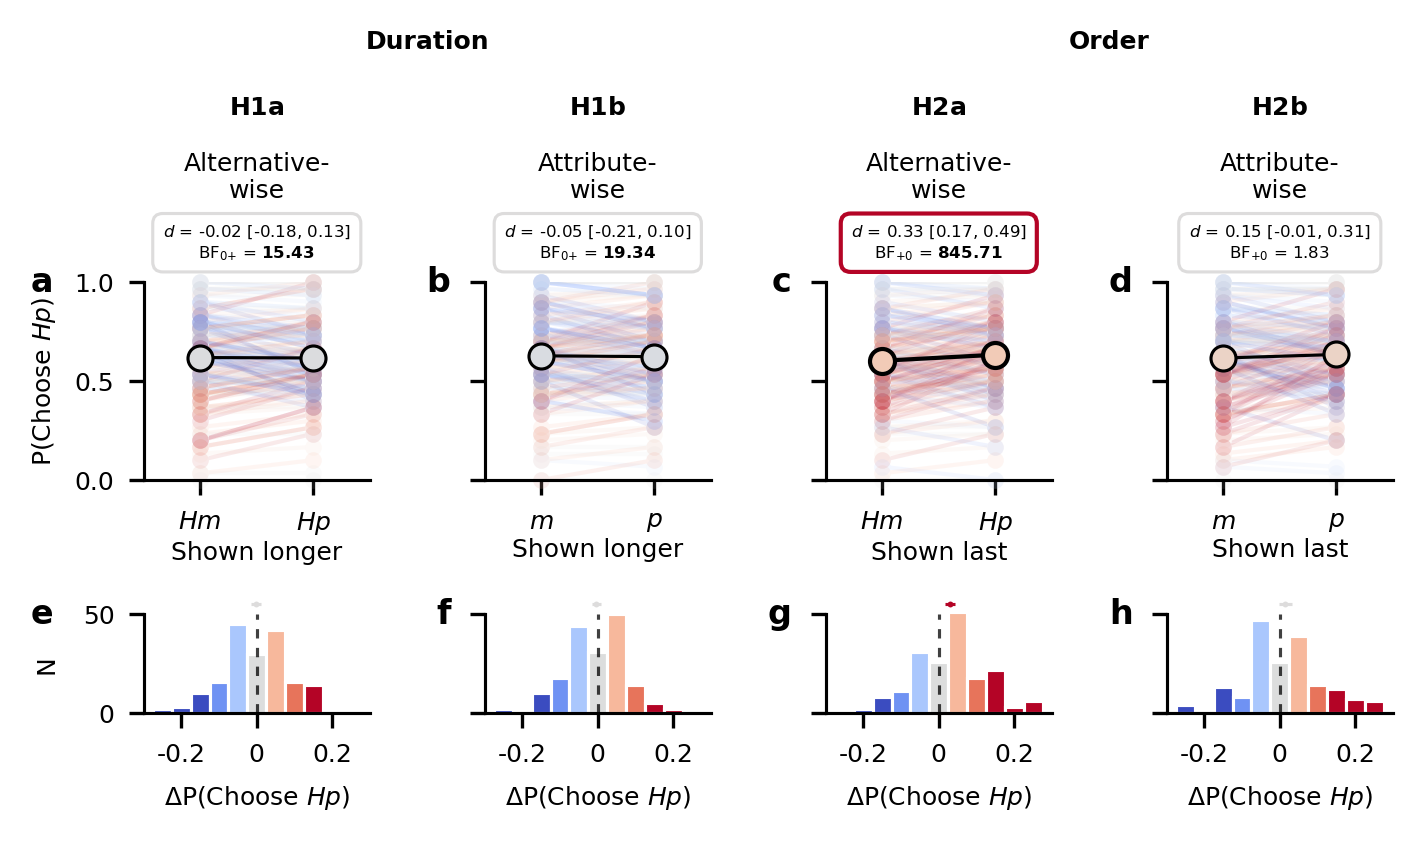
\includegraphics[width=0.9\textwidth]{figures/choice_analyses_individual_changes.png}
    \caption{\textbf{Effects of presentation duration and order on choice.} Panels \textbf{a}-\textbf{d} show individual and mean changes in choice probabilities of the higher probability alternative $Hp$, for duration (\textbf{a, b}) and order manipulations (\textbf{c, d}) in alternative- (\textbf{a, c}) and attribute-wise (\textbf{b, d}) presentation. Each semi-transparent connected pair of dots indicates choice probabilities for $Hp$ of a single participant in trials where $Hm$ vs. $Hp$ was favoured by the presentation manipulation. Group means are indicated by opaque slate dots and lines. Cohen's $d$ with HDI$_{95\%}$ obtained from paired BEST analysis, and the Bayes factors in favour of a positive directed over a null effect (BF$_{+0}$; see \nameref{sec:methods}) or its reciprocal in favour of a null effect (BF$_{0+}$) are given for each panel. Panels \textbf{e-f} show corresponding distributions of individual changes (individual slopes in panels \textbf{a-d}), with colors coding the size of individual changes. Small points and horizontal lines above histograms indicate mean and HDI$_{95\%}$ change (gray if HDI$_{95\%}$ includes 0, red if 0 is excluded).}
    \label{fig:choiceprobabilitychanges}
\end{figure*}

We hypothesized that alternatives shown longer (in alternative-wise presentation) and alternatives with better values on the attribute shown longer (in attribute-wise presentation) would be chosen more frequently. 
To this end, we computed individuals' probabilities of choosing $Hp$ when it was favoured by presentation duration (because either the alternative $Hp$ or the attribute $p$ was shown longer) and when it was not. We then used directed Bayes Factor $t$-tests to test the hypotheses of positive versus a null effects in the difference of choice probabilities (see \nameref{sec:methods}). 

On average and across presentation formats, participants chose $Hp$ with a probability of 62.0\% when it was favoured by presentation duration, and 62.3\% when it was not.
There was strong evidence against an effect of presentation duration on choice probability across presentation formats (mean difference = $-0.2\%$ $[-1.1\%, 0.6\%]$; mean $d = -0.04$ $[-0.20, 0.11]$; BF$_{{+}0} = 0.053$, BF$_{0{+}} = 18.84$).
Separate tests for each presentation format confirmed evidence against an effect of presentation duration on choice probability, with strong evidence against an effect in alternative-wise presentation (H1a; mean difference = $-0.2\%$ $[-1.5\%, 1.1\%]$; mean $d = -0.02$ $[-0.17, 0.14]$; BF$_{0{+}} = 15.43$; Figure \ref{fig:choiceprobabilitychanges}a) and strong evidence against an effect in attribute-wise presentation (H1b; mean difference = $0.4\%$ $[-1.6\%, 0.8\%]$; mean $d = -0.05$ $[-0.21, 0.10]$; BF$_{0{+}} = 19.34$; Figure \ref{fig:choiceprobabilitychanges}b). 

\subsection*{Strong evidence for effect of presentation order in alternative-wise presentation}

We furthermore hypothesized that alternatives shown last (in alternative-wise presentation) and alternatives with better values on the attribute shown last (in attribute-wise presentation) would be chosen more frequently. 
To test the marginal effect of presentation order on choice (across presentation formats), we computed the individual probabilities of choosing $Hp$ when it was favored by the last presentation stage (because either the alternative $Hp$ or the attribute $p$ was shown last) and when it was not, and performed directed Bayes factor $t$-tests and Bayesian estimation of their difference. 
Across presentation formats, participants chose the $Hp$ alternative with a probability of 63.3\% when it was favoured in the final presentation stage, and 60.9\% when it was not (Table \ref{tab:choiceprobs}).
There was extreme evidence in favour of an effect of presentation order on choice across  presentation formats (mean difference = $2.4\%$ $[1.2\%, 3.5\%]$; mean $d = 0.32$ $[0.17, 0.49]$; BF$_{{+}0} = 806.85$). 
Separate tests for each presentation format showed that the effect was more specific to alternative-wise presentation, with extreme evidence for an effect (H2a; mean difference = $3.0\%$ $[1.7\%, 4.4\%]$; mean $d = 0.33$ $[0.18, 0.49]$; BF$_{{+}0} = 845.71$; Figure \ref{fig:choiceprobabilitychanges}c). In attribute-wise presentation, evidence anecdotally favoured a positive effect (H2b; mean difference = $1.5\%$ $[0.0\%, 3.1\%]$; mean $d = 0.15$ $[-0.01, 0.31]$; 96.81\% of posterior mass above zero; BF$_{{+}0} = 1.83$; Figure \ref{fig:choiceprobabilitychanges}d).


% Discussion
% ----------
\section*{Discussion}

% Summary of the study
In this study, we investigated the causal effects of attribute- and alternative-wise presentation duration and order in two-alternative risky choice. In contrast to causal interpretations of simple gaze-dependent accumulation models, our data did not support a causal role of presentation duration in either presentation format. Instead, we found strong evidence for a causal effect of presentation order on choice, especially when information was presented alternative-wise.

% \subsection*{No effect of presentation duration}

% Prior:
Prior work has reported causal effects of viewing- and presentation duration on preferential (and perceptual) choice \parencite{shimojo2003GazeBiasBoth,armel2008BiasingSimpleChoices,parnamets2015BiasingMoralDecisions,tavares2017AttentionalDriftDiffusion,sui2020TimingGazecontingentDecision,liu2020ExploitingDynamicsEye,fisher2021IntertemporalChoicesAre} using external control of presentation durations or gaze-contingent decision prompts. In free choice paradigms, these effects are well described by gaze-dependent accumulation models like the \gls{addm}, which assume that an alternative's value representations are discounted while it is not fixated by (or presented to) the decision maker.

% Update:
In our task, evidence strongly favoured null effects of presentation duration on choice, both in alternative- and attribute-wise presentation formats.

% Posterior:
This lack of replication suggests that more work is needed to better understand the conditions under which fixation- or presentation duration can affect choice behaviour. It is possible that duration effects are moderated by specific aspects of the decision task itself, like presentation durations, and the type and delivery of choice stimuli. 

It remains, however, an experimental challenge to investigate the causal effects of different aspects of information search on choice: With the external control of presentation parameters, participants are prompted for a decision either before or after they would have made a choice in a free response paradigm. Studies experimentally controlling stimulus presentation (including studies with gaze-dependent decision prompts) thereby differ from simple decision making tasks where participants determine the time of choice themselves; their experimental manipulations interfere with and alter the natural course of decision making. Here, recent work has demonstrated an elegant possibility to induce biases in information search, with downstream effects on choice: \textcite{gwinn2019SpilloverEffectsAttentional} had participants acquire attentional biases in a separate task, which carried over to a choice task otherwise free from interference. Notably, the authors found that not gaze duration, but the location of the first fixation, mediated the effect of the attentional manipulation on choice, providing additional evidence of effects of information order on choice over viewing duration alone.

% \subsection*{Order effect}

% Prior
Regarding the association between the order of information search during decision making and choice, most eye tracking studies of decision making find the last fixation to be predominantly directed towards the chosen alternative \parencite{krajbich2010VisualFixationsComputation,krajbich2011MultialternativeDriftdiffusionModel,glickman2019FormationPreferenceRisky,stewart2016EyeMovementsRisky,fiedler2012DynamicsDecisionMaking}. This association is predicted by gaze-dependent accumulation models like the \gls{addm}, where relative evidence for an alternative is more likely to cross the decision boundary while it is fixated. Notably, however, the \gls{addm} does not imply a causal role of information order or the final fixation on choice in particular. In contrast, leaky accumulator models \parencite[e.g.,][]{glickman2019FormationPreferenceRisky,molter2021GazedependentEvidenceAccumulation,ashby2016FindingRightFit,usher2001TimeCoursePerceptual} predict that information acquired early in the trial decays, and the relative weight of more recent information is increased.

% Update:
We found strong evidence for a causal effect of presentation order, so that information presented last influences decisions more than information presented earlier. This recency effect was particularly strong in the alternative-wise presentation format.

% Posterior:
Our results thereby support theories of gaze-dependent accumulation which include a form of accumulation leak and can account for causal recency effects. Interestingly, prior work has identified recency effects in decisions from experience and related paradigms, where information about risky alternatives' outcomes is actively sampled by the decision maker, and therefore also acquired sequentially \parencite{hertwig2004DecisionsExperienceEffect,tsetsos2012SalienceDrivenValue}. Our results suggest that a similar, and causally directed effect is present during decisions from description, where stimulus information is also experienced sequentially.

One possible explanation for the observed recency effect is that decision makers have imperfect memory about the stimulus information (potentially reinforced by the fast-paced presentation) and then base their choice on more recent, better remembered information. This would constitute a memory-bias within single trials, similar to previously described effects on longer timescales \parencite{gluth2015EffectiveConnectivityHippocampus,weilbacher2021InfluenceVisualAttention}.

Our results further provide evidence that the observed association between decision makers' last fixation and choice goes beyond simple "confirmation" or response locking explanations assuming that choices are already determined before the final fixation and response is made.

%\subsubsection*{Possible confound of duration and order in prior work}

In addition to the last fixation preferably being directed to the chosen alternative, eye tracking studies of decision making typically find longer gaze towards the chosen alternative \parencite{shimojo2003GazeBiasBoth,fiedler2012DynamicsDecisionMaking,krajbich2010VisualFixationsComputation,krajbich2011MultialternativeDriftdiffusionModel,glickman2019FormationPreferenceRisky,cavanagh2014EyeTrackingPupillometry,stewart2016EyeMovementsRisky,molter2021GazedependentEvidenceAccumulation}. Both being associated with choice, these two variables might be confounded frequently, that is, alternatives that are looked at last are also looked at longer during the decision. Consequently, the effects of duration and order can be mistaken for each other, without explicit control.
This issue can also occur in experimental designs using gaze-dependent decision prompts, as – depending on the specific conditions triggering the prompt – the last fixation is potentially more likely to be directed at the alternative determined to receive longer gaze.

%\subsection*{Implications for the design of choice situations}

While prior work demonstrated that random or externally induced fluctuations in visual attention can have downstream effects on choice mainly through viewing duration, our work highlights the importance of the temporal order in which information is encountered. This suggests that, in situations where presentation order can be controlled, such as television-, cinema- or online video advertisements, choices could be systematically shifted towards certain alternatives. We note, however, that these settings typically do not involve the need to choose (as in our experiment). Yet, it is conceivable that for those cinema-goers who already decided to buy ice-cream, still deliberating which flavour to get, choices are shifted towards the flavour presented last (and closest to their buying decision) in the advertisement clip. Desired (e.g., healthful) choices could then be promoted by reminding decision makers of them just before choices are made.

Similarly, \textcite{sullivan2021HealthfulChoicesDependa} argued in favour of time-dependent interventions to promote healthful food choices, as they found health information to enter the decision process with a longer latency than taste information. Reducing overall time pressure could increase healthful choices by reducing the gap in attribute latencies. Alternatively, they suggest that showing health-related information \emph{first} should decrease the latency gap and thereby promote healthy choices. Our results highlight the opposite direction: Attribute-information shown first to participants reduced participants' likelihood of choosing alternatives with better values on that attribute. Note that our study addressed primacy and recency effects on the same one-dimensional construct. We therefore cannot distinguish positive recency- from negative primacy effects, as information shown last was by design \emph{not} shown first. Future work could address possible independent contributions of both effects.

A possible explanation for these apparent differences, apart from the different goods being chosen, is that the latency construct in the model by \textcite{sullivan2021HealthfulChoicesDependa} might be more related to consideration \emph{duration} than \emph{order}: Attributes with lower latencies can, by definition, influence the decision process for a longer duration than others. This way, the order and duration effects are inherently linked in their model.

% \subsection*{Conclusion}

In conclusion, we showed that presentation order but not presentation duration had a causal effect on risky choice behaviour, in an external presentation paradigm. This has important implications for theories of decision making, which should incorporate mechanisms like accumulation leak, to account for observed recency effects, and suggests an important role of the presentation order – particularly the information presented just before a choice is made – in real world decisions.

% Methods
% =======
%TC:ignore
\section*{Methods}
\label{sec:methods}

All data collection and analysis procedures were preregistered on the Open Science Framework ahead of data collection \parencite{molter2021InvestigatingCausalEffects}.

\subsection*{Participants}
\label{methods:participants}
The experiment was conducted online and participants were recruited via the platform Prolific.co. Our target sample size was 200 participants. We accepted entries on the Prolific platform until 200 complete submissions were reached. Sample size was determined to exceed that of previous laboratory-based experiments addressing related questions \parencite[e.g.,][]{armel2008BiasingSimpleChoices,liu2020ExploitingDynamicsEye,parnamets2015BiasingMoralDecisions,sui2020TimingGazecontingentDecision,fisher2021IntertemporalChoicesAre}, accounting for the possibility of lower quality data due to the online setting. 
Participants were paid £3.75 for completing the study, which took around 30 minutes. They had the chance to win a bonus amount ranging from £0 to £9.85, as one of their chosen gambles was randomly determined and played out after the experiment. The experiment included webcam-based eye tracking (see \nameref{sec:supplement}), so only participants with a working webcam using Google Chrome or Mozilla Firefox could participate.
Participants gave informed consent prior to participation in the study.

Participants were excluded from the analysis without replacement if one of the following criteria was met: i) The participant chose a dominated alternative more than 4 times (20\% of catch trials, see below). ii) The participant reported to be red-green colorblind or having difficulty distinguishing the colors in the task. iii) The participant reported having technical difficulties that prevented them from diligent execution of the task. iv) The participant's self-reported decision strategy suggested that task instructions were misunderstood. v) The participant reported nonserious participation in the task \parencite{aust2013SeriousnessChecksAre}.

Twenty-one participants were excluded from the analyses (16 for criterion 1, four for criterion 2, one for criterion 4), resulting in a final sample size of 179 (mean $\pm$ s.d. age = 32.46 $\pm$ 13.85; 84 females, 94 males, one other).

\subsection*{Behavioral task}
\label{sec:methods:task}

Participants performed a binary sequential presentation risky choice task, where they made repeated incentivized choices between two graphically displayed all-or-nothing gambles (Figure \ref{fig:taskstimuli}). Each gamble represented the chance to win a monetary amount $m$ with a probability $p$ and nothing otherwise. Winning amounts $m$ were represented by partially filled bars (a fully filled bar represented an amount of 10\pounds), and winning probabilities $p$ by pie charts. Each trial was divided into a presentation phase and a choice phase. During the presentation phase, participants learned about the two available gambles' attributes. Information was presented sequentially. There were two types of presentation: Alternative-wise and attribute-wise presentation.

In trials with alternative-wise presentation (Figure \ref{fig:taskstimuli}a) both attributes of one gamble were shown simultaneously, followed by both attributes of the other gamble. In trials with attribute-wise presentation (Figure \ref{fig:taskstimuli}b), one attribute (e.g., winning probability $p$) of both gambles was presented simultaneously, followed by the other attribute (e.g., amount $m$) of both gambles. Presentation always alternated two times between alternatives or attributes (i.e., A-B-A-B). Crucially, one alternative (in trials with alternative-wise presentation) or attribute (in trials with attribute-wise presentation) in each trial was selected to be the target and shown longer than the other one. Target attributes or alternatives were always presented for 1500 ms, whereas other alternatives or attributes were presented for 1000 ms, resulting in a final presentation time advantage for the target of 1000 ms (2x 1500 ms vs. 2x 1000 ms).

After the presentation phase, stimulus information was hidden and participants were prompted to make a choice between the two alternatives within 3 seconds.
After completing all choice trials, one gamble chosen by the participant in a randomly determined trial was played out for a real bonus payment.
The task can be run at \url{https://moltaire.github.io/causality_task}.

All participants made choices for the same 140 choice  problems (see below) divided into two blocks. Trial order in each block and the horizontal position of the alternatives in each trial was randomized. Block order was counterbalanced between participants.

\subsection*{Stimuli}
\label{sec:methods:stimuli}

We created a set of 15 core choice problems including one alternative with a higher probability of winning a lower amount ($Hp$) and one alternative with a lower probability of winning a higher amount ($Hm$). Choice problems were created algorithmically to cover most of the attribute space, be maximally different from each other, and be diagnostic of different risk attitudes. For this last criterion, we controlled the $\alpha$ values for which two alternatives in a pair would have equal expected utility (using a standard power utility function). The distribution of these indifference-implied $\alpha$ values is shown in in Figure \ref{fig:taskstimuli}d. Core choice problems are illustrated in Figure \ref{fig:taskstimuli}c.

Then eight trials were created for each core problem by fully crossing the factors (i) presentation format (alternative-wise vs. attribute-wise), (ii) target alternative / attribute ($Hp$ vs. $Hm$; $p$ vs. $m$), and (iii) presentation order (target first and third vs. second and last). This resulted in a total of 120 experimental choice trials. 

We added 20 catch trials with one dominant alternative for a total of 140 trials (Figure \ref{fig:taskstimuli}e). In catch trials, individual presentation durations were set to 1250 ms, resulting in the same overall presentation duration (5000 ms), but no presentation time advantage for any alternative or attribute.


\subsection*{Statistical modelling}
We performed a Bayesian logistic regression analysis of choice behavior, with choice ($Hp$ vs. $Hm$) as the dependent variable and the following predictors: Expected value difference ($EV_{Hp} - EV_{Hm}$; z-scored), presentation format (by-attribute vs. by-alternative; effect-coded), duration-favored ($Hp$ favored vs. $Hm$ favored by duration manipulation; effect-coded), last-stage-favored ($Hp$ favored vs. $Hm$ favored in last presentation stage; effect-coded), and interaction terms between presentation format and duration-favored and last-stage-favored. The model included random intercepts and slopes over participants and used the default priors set by the bambi library \parencite{westfall2017StatisticalDetailsDefault}.

We performed directed Bayes factor (BF) $t$-tests \parencite{morey2011BayesFactorApproaches} of our main hypotheses, testing the directed hypotheses that differences in choice probabilities are larger than zero, over a point null hypothesis. All Bayes factor $t$-tests used default JZS priors (Cauchy distributed with scale $r = \sqrt{2}/2$) implemented in the BayesFactor package \parencite{morey2018BayesFactorComputation}.

Additionally, we ran paired Bayesian estimation \parencite[BEST;][]{kruschke2013BayesianEstimationSupersedes,kruschke2014DoingBayesianData} analyses to compute mean differences, effect sizes $d$ and associated 95\% highest posterior density intervals (HDI$_{95\%}$).

We ran two chains with 5000 samples each after a tuning phase of 1000 samples for all BEST analyses and the Bayesian mixed-effects model. Convergence was diagnosed visually and by means of the Gelman-Rubin statistic ($|1 - \hat{R}| \le 0.05$ for all chains).

We determine parameters in the regression and BEST analyses to be credibly different from zero if HDI$_{95\%}$ exclude zero or at least 95\% of the posterior mass is above (below) zero.
For interpretation of Bayes factors' evidence strength, we follow the conventional categorization based on \textcite{jeffreys1998TheoryProbability}: Anecdotal (1 $<$ BF $<$ 3); Moderate (3 $\le$ BF $<$ 10); Strong (10 $\le$ BF $<$ 30); Very strong (30 $\le$ BF $<$ 100); Extreme (100 $\le$ BF).


\subsection*{Software}
The task was programmed in jsPsych \parencite{deleeuw2015JsPsychJavaScriptLibrary}. Webcam-based eye tracking was implemented using the webgazer.js library \parencite{papoutsaki2016webgazer}.
Data processing and analyses were done in Python with numpy \parencite{harris2020array} and pandas \parencite{mckinney2012PythonDataAnalysis} libraries. Bayesian analyses were implemented in PyMC3 \parencite{salvatier2016ProbabilisticProgrammingPython}, mixed models used bambi \parencite{capretto2021BambiSimpleInterface}. Bayes Factor $t$-tests were performed using the R package BayesFactor \parencite[]{morey2018BayesFactorComputation}. Figures were created using matplotlib \parencite{hunter2007Matplotlib2DGraphics}.

\subsection*{Data and code availability}
All raw and preprocessed data and scripts to reproduce all processing and analyses steps and figures are available at \url{https://github.com/moltaire/gaze-choice-causality}.
%TC:endignore

%TC:ignore
% Adjust to smaller font size
% ---------------------------
\renewcommand*{\bibfont}{\small}
\printbibliography

\subsection*{Author contributions}

Conceptualization: F.M. and P.N.C.M. Data curation: F.M. Formal analysis: F.M. Funding acquisition: P.N.C.M. Investigation: F.M. Methodology: F.M. Project administration: P.N.C.M. Resources: F.M. Software: F.M. Supervision: P.N.C.M. Validation: F.M. Visualization: F.M. Writing - original draft: F.M. Writing - review \& editing: F.M. and P.N.C.M.

\subsection*{Competing Interests Statement}

The authors declare no competing interests.

\clearpage

% Supplementary Information
% -------------------------
\section*{Supplementary Information}
\label{sec:supplement}

\renewcommand{\thefigure}{S\arabic{figure}}
\setcounter{figure}{0} 

\renewcommand{\thetable}{S\arabic{table}}
\setcounter{table}{0} 

\subsection*{Webcam-based eye tracking}
\label{sec:eye-tracking}

% MAYBE: Include figure showing valid and invalid validation blocks, histogram of sampling rates and / or errors?

Participants' gaze during the task was recorded using webcam-based eye tracking implemented in the JavaScript library webgazer.js \parencite{papoutsaki2016webgazer,yang2020WebcambasedOnlineEyetracking}. To this end, the task included a webcam setup at the start of the experiment, a 13-point calibration routine, and a 5-point validation routine before the start of each block, where participants were instructed to focus their gaze on indicated screen locations for three seconds. Validation points were chosen to correspond to the locations where stimulus information would be presented during experimental choice trials.

We assessed the quality of the collected eye tracking data using multiple complementing metrics: First, we measured the sampling rates obtained in each validation, which heavily depend on the device that runs the experimental task. Mean $\pm$ s.d. sampling rates were 15.96 $\pm$ 7.95 Hz and ranged from 0.49 Hz to 29.55 Hz, and 71\% of blocks had sampling rates above 10 Hz during validation.

Second, as a measure of bias, we computed the average absolute distance of the estimated gaze location samples from the corresponding validation targets in x- and y directions (in percent of screen width and height, respectively). Mean $\pm$ s.d. error (clustered by block) was 5.58 $\pm$ 7.11\% in x- and 8.79 $\pm$ 9.76\% in y-direction. 

Third, as a measure of accuracy, we computed the sample variability as the standard deviation of samples corresponding to a single validation target in x- and y-directions. Mean $\pm$ s.d. variability was 5.81 $\pm$ 3.07\% in x- and 7.46 $\pm$ 4.70\% in y-direction. 

Fourth, we computed the proportion of samples within an elliptical \gls{aoi} around the corresponding validation target. For this, we set the \gls{aoi}-width and -height to 15\% of the screen width and height, respectively (note that widths and heights of 25\% would leave no white space between \glspl{aoi} due to the stimulus spacing used in the task). On average, only 51.80 $\pm$ 26.12\% of the samples were contained within a validation target's \gls{aoi}.

Next, we set minimum thresholds on each of these parameters to classify validation results as valid or invalid: We required a minimum sampling rate of 10 Hz, a maximum average error and a maximum variability of 20\% in x- and y-directions, and a minimum of 60\% of samples within the validation target \gls{aoi}. Only 33 of 356 blocks (9.27\%) fulfilled these minimal quality requirements. In addition, it can be assumed that eye tracking quality only \emph{decreased} during a block, due to head movement or other sources of variability (e.g., changes in lighting conditions, etc.). We therefore did not perform any further explorative analyses on the eye tracking data. We note that it might be possible to correct for systematic biases in validation (e.g., using clustering approaches). Future studies could benefit from improved webcam-based eye tracking data by performing online checks of validation accuracy and repeating calibration and validation steps until an acceptable level of quality is reached.

\subsection*{Influence of presentation format on value integration}

Our preregistration contained the additional hypothesis that presentation format (alternative- vs. attribute-wise presentation) elicits different forms of value integration in the decision process. Specifically, we hypothesized, that alternative-wise presentation would elicit more integrative, within-alternative processing, whereas attribute-wise presentation would be associated with more comparative processing within attribute dimensions and between alternatives.
To test this hypothesis, we fit two behavioral models, which used within-alternative and within-attribute integration of attributes, respectively, to the choice and response time data of each participant. Crucially, the models were fit separately for trials with alternative- and attribute-wise presentation. We then computed the relative fit of the models for each participant and presentation format by taking the difference of the models’ \gls{bic} \parencite{schwarz1978EstimatingDimensionModel}. Finally, we performed directed paired Bayes factor $t$-tests of the differences, testing the directed hypothesis that the relative fit of the within-alternative integration model over the between-alternative model is increased in alternative-wise vs. attribute-wise presentation.

\subsubsection*{Behavioural modelling}

We analyzed participants' choice and response time data using two different behavioral models. Both models shared a similar general structure: During the presentation phase of the trial, a relative evidence signal $R$ is assumed to be formed (Figure \ref{fig:models}a-b), depending on the presentation format, duration, and order. After the choice prompt, a noisy diffusion process between two decision bounds (corresponding to choosing $Hp$ and $Hm$, respectively) is initiated that elicits a choice at a time point $t$ (Figure \ref{fig:models}c). Crucially, the drift rate of the diffusion process is proportional to the relative evidence signal $R$ at the end of the presentation phase. For both models, the diffusion process after the choice prompt is parameterized by a drift constant $v$ (that scales the final relative evidence signal $R$), a noise parameter $s$, while the boundary separation is kept constant at a value of 1.
The two models only differed in the process of calculating the relative evidence signal $R$ during the presentation phase.

\paragraph{Alternative-wise integration model}
The alternative-wise integration model (slate-gray in Figure \ref{fig:models}) computes alternative-wise expected utilities, using a standard utility function ($U_i=p_i m_i^\alpha$). During the presentation phase, the difference between the expected utilities is assumed to accumulate over time. Critically, the momentarily not presented alternative’s utility is discounted by an alternative-wise gaze-discount $\theta$. The final relative evidence signal $R_{altwise}$ is given by
$$R_{altwise} =g_{Hp} (U_{Hp}- \theta U_{Hm} ) + g_{Hm} \theta U_{Hp}-U_{Hm})$$
Where $g_{Hp}$ and $g_{Hm}$ are the relative presentation durations of $Hp$ and $Hm$. Note that in trials with attribute-wise presentation, $g_{Hp}$ and $g_{Hm}$ are set to 0.5, as both alternatives’ attributes are presented equally long.
Additionally, the model uses a parameter $b_{last}$ to predict order effects in trials with alternative-wise presentation: Positive $b_{last}$ shift $R$ towards the last-presented alternative, negative $b_{last}$ shift it to the alternative presented first.

\paragraph{Attribute-wise integration model}
The attribute-wise model (orange in Figure \ref{fig:models}) assumes that the relative evidence $R$ is computed through attribute comparisons between alternatives, weighted addition of attribute differences, and accumulation of differences over time. Importantly, it assumes that the momentarily not presented attributes are discounted by an attribute-wise gaze-discount $\eta$. The final relative evidence signal $R_{attwise}$ is given by
\begin{align*}
R_{attwise} = & g_p (w_p \Delta_p + \eta (1 - w_p) \Delta_m ) + \\
              & g_m (\eta w_p \Delta_p + (1 - w_p ) \Delta_m )
\end{align*}
Where $\Delta_p$ and $\Delta_m$ are the attribute differences between $Hp$ and $Hm$ alternatives. $g_p$ and $g_m$ are relative presentation durations for $p$ and $m$ attributes, respectively. $w_p$ controls the relative weighting between probability and outcome attributes. Note that attributes are also normalized in each trial (by dividing by the sum of values on the attribute). During trials with alternative-wise presentation, the relative gaze durations towards attributes are set to 0.5, since at every point during the presentation phase, information of both attributes is presented. 
Additionally, the model uses a parameter $b_{last}$ to predict order effects in trials with attribute-wise presentation: Positive $b_{last}$ shift $R$ towards the alternative with the higher value on the last-presented attribute, negative $b_{last}$ shift it to the alternative with the higher value on the alternative presented first.

% Figure: Behavioural models
\begin{figure*}[t]
    \centering
    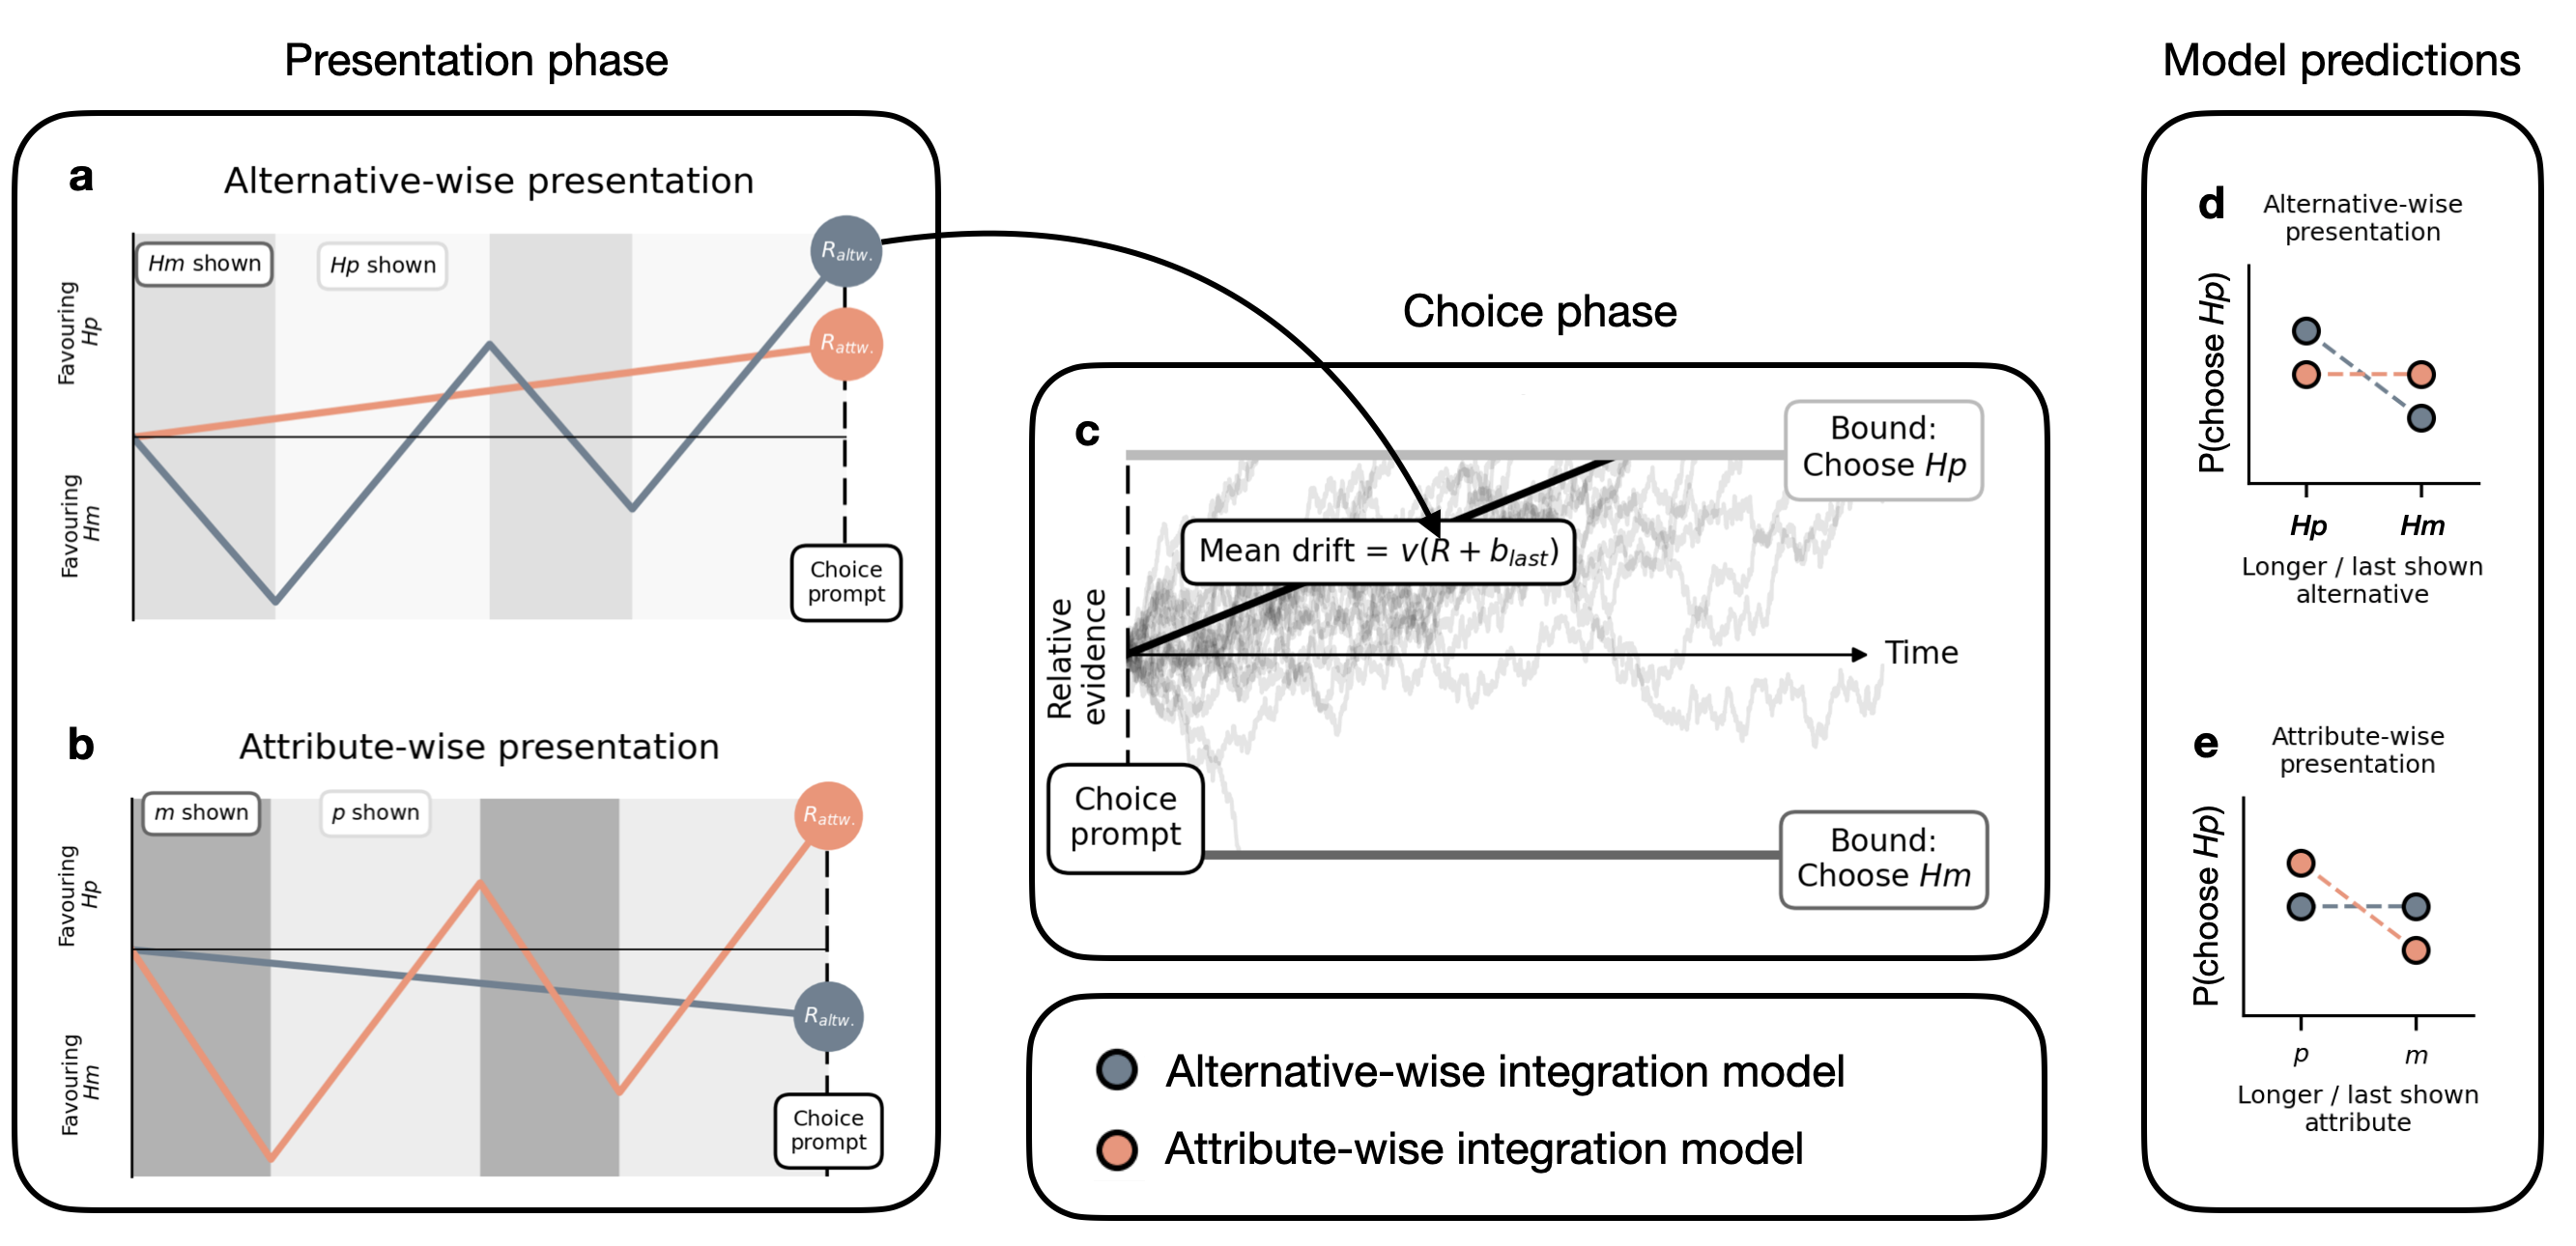
\includegraphics[width=0.9\textwidth]{figures/behavioural_models.png}
    \caption{\textbf{Behavioural models and their predictions.} \textbf{a)} Construction of drift-rates in trials with alternative-wise presentation. Only the alternative-wise model’s drift rate is sensitive to effects of presentation duration in alternative-wise presentation. Analogously, only the alternative-wise model produces order effects in alternative-wise presentation, controlled by the $b_{last}$  parameter. \textbf{b)} Construction of drift rates in attribute-wise presentation. Here, only the attribute-wise model’s drift rate is sensitive to effects of presentation duration. Similarly, only the attribute-wise model produces order effects in attribute-wise presentation, controlled by the $b_{last}$ parameter. \textbf{c)} After construction of the drift rate in the presentation phase, choices and response times result from a diffusion process with the previously constructed drift rate. \textbf{d-e)} Both models’ predicted effects of alternative-wise (\textbf{d}) and attribute-wise (\textbf{e}) presentation duration. Slate-gray color refers to alternative-wise model. Orange color refers to attribute-wise model.}
    \label{fig:models}
\end{figure*}

\paragraph{Parameter estimation}
Both models were implemented in pyddm \parencite{shinn2020FlexibleFrameworkSimulating} with a temporal resolution $dt$ = 0.01, and a resolution of the evidence space $dx$ = 0.01. 
Both models were fit separately to trials with alternative-wise and attribute-wise presentation using pyddm’s default differential evolution algorithm, minimizing the Bayesian Information Criterion \parencite[BIC;][]{schwarz1978EstimatingDimensionModel}.

\paragraph{Model validation}
To ensure interpretability and validity of the models’ parameter estimates, we performed a parameter recovery study as follows: First, we estimated each model’s parameters from the empirical data of each participant. Then we simulated a synthetic data set of the same size as the empirical one, using the individually obtained estimates. Then we re-fit the models to the synthetic data and compared known generating to the obtained recovered parameters by means of Bayesian linear regression (dependent variable: recovered parameter; independent variables: Intercept, generating parameter) and correlation analyses \parencite{kruschke2013BayesianEstimationSupersedes,lee2013BayesianCognitiveModeling}. The models' parameters could be recovered to a satisfying degree, with the gaze-discount parameters $\theta$ and $\eta$ showing the largest differences (Figure \ref{fig:modelingparameterrecovery}).

Similarly, we performed model recovery analyses by fitting each model to the synthetic data generated from all models. Then, for each generating model, we performed Bayesian model selection \parencite{rigoux2014BayesianModelSelection,stephan2009BayesianModelSelection} to identify the most likely generating model. The models could be recovered almost perfectly (Figure \ref{fig:modelingmodelrecovery}).

\subsubsection*{Results}

\begin{figure*}[htbp]
    \centering
    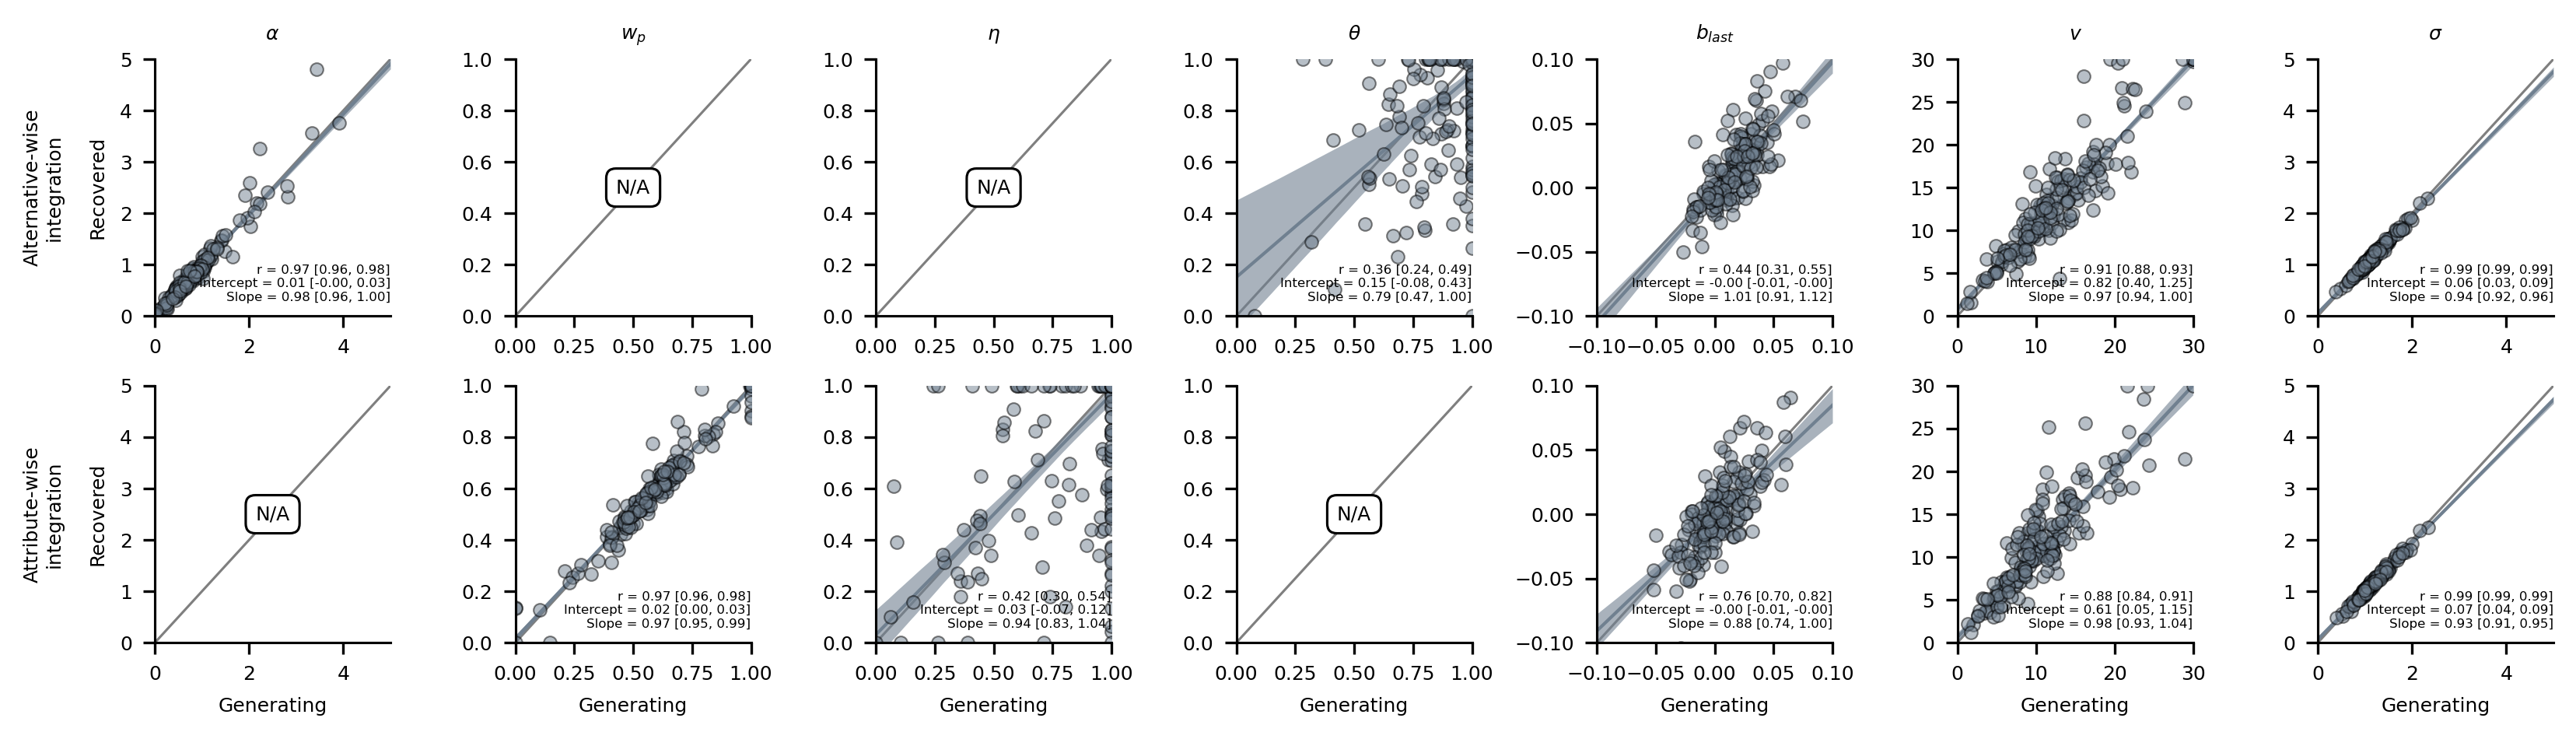
\includegraphics[width=\textwidth]{figures/ddm_recovery_parameters.png}
    \caption{\textbf{Parameter recovery of the two diffusion models.} Each panel shows the relationship between true data generating, and recovered parameter values for a single model parameter. Upper and lower rows show results from the \emph{alternative-wise} and \emph{attribute-wise} integration models, respectively. Generating parameters were obtained from fitting the models to the empirical data. Annotations report Bayesian correlation coefficient $r$, and the slope and intercept estimates of a Bayesian regression analysis with HDI$_{95\%}$ given in brackets. Perfect, unbiased recovery would show an intercept of 0 and a slope of 1, with all points on the diagonal.}
    \label{fig:modelingparameterrecovery}
\end{figure*}

\begin{figure}[htbp]
    \centering
    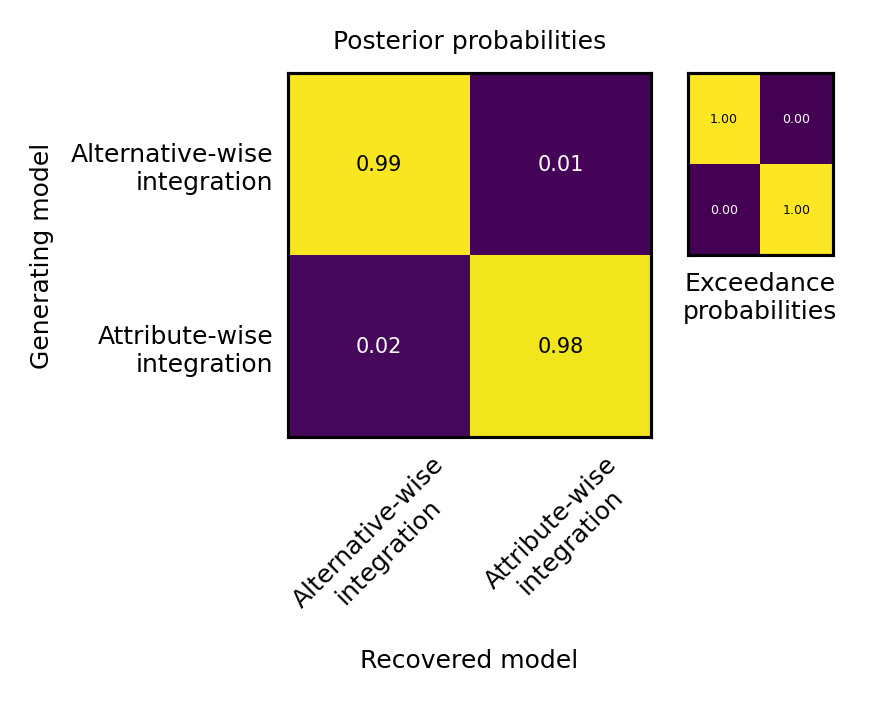
\includegraphics[width=\linewidth]{figures/ddm_recovery_models.png}
    \caption{\textbf{Model recovery results.} The large panel shows a confusion matrix from the model recovery analysis. Each cell shows the posterior model probability of a fitted model (in each column) for a given generating model (in each row). Perfect recovery would show only values of 1 on the diagonal. The smaller confusion matrix shows exceedance probabilities, analogously.}
    \label{fig:modelingmodelrecovery}
\end{figure}

% Report results of preregistered analysis
For trials with alternative-wise presentation, the mean $\pm$ s.d. \gls{bic} of the alternative-wise model was 102.16 $\pm$ 56.19 (range -24.20 to 344.44). Mean $\pm$ s.d. \gls{bic} of the attribute-wise model was 93.27 $\pm$ 57.03 (range -45.06 to 338.90), indicating a better fit of the attribute-wise model in alternative-wise presentation.

Conversely, in trials with attribute-wise presentation, the mean $\pm$ s.d. \gls{bic} of the alternative-wise model was 90.97 $\pm$ 55.24 (range -45.39 to 310.33), while the attribute-wise model achieved mean $\pm$ s.d. \gls{bic} of 97.41 $\pm$ 55.36 (range -50.91 to 321.62), indicating better fit of the alternative-wise model.

Next, we took the difference between \gls{bic} of the models for each participant and presentation format and tested whether they credibly differed from zero, using a directed paired Bayes factor $t$-test (and BEST analysis to obtain estimates of the effect size $d$). 
Results strongly supported a result \emph{opposite} to our hypothesis, namely, that the attribute-wise model was favoured in alternative-wise presentation, while the alternative-wise model was favoured in attribute-wise presentation (mean \gls{bic} difference = -15.34 [-14.57, -16.20]; mean $d$ = 2.75 [2.29, 3.23]; BF$_{{+}0}$ = 0.0011, BF$_{0{+}}$ = 907.95).

In sum, these results are contrary to our preregistered hypothesis: In trials with alternative-wise presentation, the simpler attribute-wise model was preferred. Vice versa, in trials with attribute-wise presentation, the simpler alternative-wise model was preferred.
 
% Report concerns about preregistered analysis
We note, however, that the preregistered analysis could not address our hypothesis optimally for multiple reasons. First, model complexity differed systematically between conditions: In trials with alternative-wise presentation, the alternative-wise model uses two free parameters more than the attribute-wise model (namely, the alternative-wise gaze discount $\theta$, and the alternative-wise $b_{last}$ parameter), while the reverse is true in trials with attribute-wise presentation. While the \gls{bic} takes model complexity into account, this issue highlights that the models differ in more aspects than their value-integration process (namely, the different gaze discounts and last-stage effects), prohibiting conclusions about changes in value-integration. Furthermore, more complex models are penalized for their inclusion of duration-dependent gaze-discount mechanisms to explain associations of presentation duration and choice, which our behavioural analyses showed to be absent in our data.
%TC:endignore
\end{document}
